\documentclass[11pt, oneside]{article} 
\usepackage{geometry}
\geometry{letterpaper} 
\usepackage{graphicx}
	
\usepackage{amssymb}
\usepackage{amsmath}
\usepackage{parskip}
\usepackage{color}
\usepackage{hyperref}

\graphicspath{{/Users/telliott_admin/Tex/png/}}
% \begin{center} 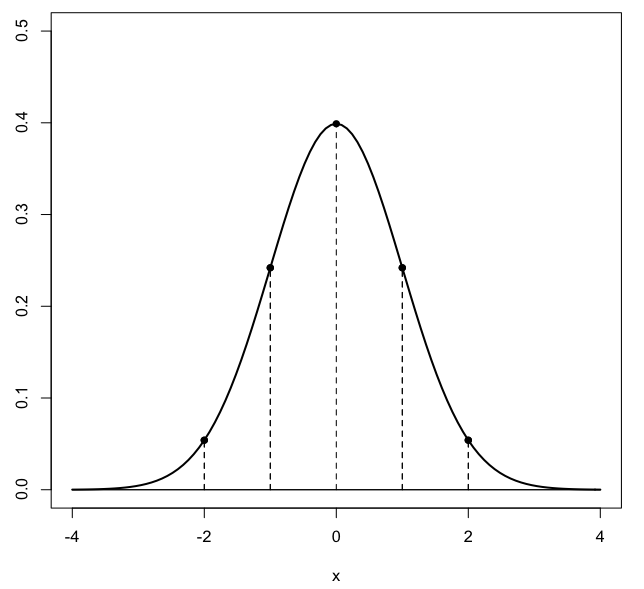
\includegraphics [scale=0.4] {gauss3.png} \end{center}

\title{Cauchy-Riemann Equations}
\date{}

\begin{document}
\maketitle
\Large

\section*{More proofs of CRE}
\subsection*{difference quotient}

We gave a first proof in the section on differentiation which goes as follows.  The derivative $f'(z)$ is defined to be the limit of the following difference quotient, if the limit exists.
\[ f'(z) = \lim_{\Delta z \rightarrow 0} \frac{f(z + \Delta z) - f(z)}{\Delta z} \]
The difference quotient is rewritten in terms of $u$ and $v$ as:
\[ \frac{u(x + \Delta x, y + \Delta y) + i v(x + \Delta x, y + \Delta y) - u(x) - i v(y)}{x + \Delta x + y + \Delta y} \]
Then we consider two special cases, one where $\Delta y = 0$ and a second where $\Delta x = 0$.  The first case yields
\[ f'(z) = u_z + i v_x \]
and the second yields
\[ f'(z) = -i u_y + v_y \]
The derivative is required to be the same for all directions of approach to the point, so we can equate the two expressions
\[ u_x + i v_x = -i u_y + v_y \]
Since both the real and the imaginary parts must be equal, we obtain the CRE:
\[ u_x = v_y \]
\[ u_y = - v_x \]

\subsection*{chain rule}
Here is a second approach:

Write:
\[ z = x + iy \]
Clearly,
\[ \frac{\partial z}{\partial x} = 1 \]
\[ \frac{\partial z}{\partial y} = i \]
Now,
\[ w = f(z) \]
\[ = u(x,y) + i \ v(x,y) \]
where $u$ and $v$ are real functions over $\mathbb{R}^2$.

Recalling the chain rule
\[ w = u(x,y) + i \ v(x,y) \]
\[ \frac{\partial w}{\partial x} = \frac{dw}{dz} \ \frac{\partial z}{\partial x} \]
\[ =  \frac{dw}{dz} \]
(by the result immediately above, that $\partial z/\partial x = 1$).
Similarly
\[ \frac{\partial w}{\partial y} = \frac{dw}{dz} \ \frac{\partial z}{\partial y} \]
\[ =  i \frac{dw}{dz} \]
Hence we can equate the two expressions for $dw/dz$:
\[ \frac{dw}{dz} = \frac{\partial w}{\partial x} = -i \frac{\partial w}{\partial y} \]

Now if we actually compute the partials and plug them in to the last equation, we obtain:
\[ \frac{\partial w}{\partial x} = u_x + i v_x \]
\[ \frac{\partial w}{\partial y} = u_y + i v_y \]
\[ u_x + i v_x = -i (u_y + i v_y) = v_y - i u_y \]
Both the real and the imaginary parts must be equal:
\[ u_x = v_y \]
\[ v_x = - u_y \]
These are (again) the CRE.

It is worth taking a breath for a moment and repeating what we just said:  the derivative of a differentiable complex function $z$ (that is, an analytic function) is
\[ \frac{df}{dz} = \frac{\partial f}{\partial x} = - i \frac{\partial f}{\partial y} \]
\[ = u_x + i v_x \]
\[ = -i (u_y + i v_y) \]
\[ = v_y - i u_y\] 

\subsection*{Alder}
A third, very simple proof is given in Alder:

Suppose $f: C \rightarrow C$ is a function, taking $x+iy$ to $u(x,y) + iv(x,y)$, then the derivative is a matrix of partial derivatives:
\[
\begin{matrix}
u_x &  u_y \\
v_x & v_y
\end{matrix}
\]

.. the above matrix is the two dimensional version of the slope of the tangent line in dimension one.  It gives the linear part (corresponding to the slope) of the affine map which best approximates $f$ at each point.

.. if $f$ is differentiable in the \emph{complex} sense, this must be just a linear complex map, i.e. it multiplies by some complex number.  So the matrix must be in our set of complex numbers.  In other words, for every value of $x$ it looks like
\[
\begin{matrix}
a & -b \\
b &  \ \ a
\end{matrix}
\]
for some real numbers $a,b$, which change with $x$.

Of course, this constraint leads directly to the CRE.

A very important point is that the CRE and analyticity and differentiability are all related  (either a function has all these properties or none of them).  For an analytic function, the rules for integration and differentiation are analogous to the real case.  For example:
\[ \int \frac{1}{3} z^2 \ dz = z^3 \]
\[ \frac{d}{dz} \ \frac{1}{z - z_0} = - \frac{1}{(z-z_0)^2} \]
We will see a lot more of this.

\subsection*{McMahon}
Here is yet another proof which I found in McMahon.  I am not 100\% confident about it, but I include it here because it explains Shankar's statement that by definition an analytic function has no dependence on $z*$.  (The $\bar{z}$ notation is used below).

Write
\[ z = x + iy , \ \ \  \bar{z} = x - iy \]
so
\[ x = \frac{1}{2} (z + \bar{z}) , \ \ \ y = \frac{1}{2i} (z - \bar{z}) \]

Take partial derivatives:
\[ \frac{\partial x}{\partial z} = \frac{1}{2} = \frac{\partial x}{\partial \bar{z}} \]
\[ \frac{\partial y}{\partial z} = \frac{1}{2i} = -\frac{i}{2} = -\frac{\partial y}{\partial \bar{z}} , \ \ \ \frac{\partial y}{\partial \bar{z}} = \frac{i}{2} \]

Then, using the chain rule we write:
\[ \frac{\partial}{\partial z} =  \frac{\partial x}{\partial z}  \frac{\partial}{\partial x} + \frac{\partial y}{\partial z}  \frac{\partial}{\partial y} = \frac{1}{2} \ [ \ \frac{\partial}{\partial x} - i \frac{\partial}{\partial y} \ ] \]
\[ \frac{\partial}{\partial \bar{z}} =  \frac{\partial x}{\partial \bar{z}}  \frac{\partial}{\partial x} + \frac{\partial y}{\partial \bar{z}}  \frac{\partial}{\partial y} = \frac{1}{2} \ [ \ \frac{\partial}{\partial x} + i \frac{\partial}{\partial y} \ ] \]

Now apply the two operators (just a matter of a few minus signs):
\[ \frac{\partial f}{\partial z} =  \frac{1}{2} \ [ \ \frac{\partial}{\partial x} - i \frac{\partial}{\partial y} \ ]  \ [ \ u + iv \ ] = \frac{1}{2} \ [ \ (u_x + v_y) + i( v_x - u_y) \ ] \]
\[ \frac{\partial f}{\partial \bar{z}} =  \frac{1}{2} \ [ \ \frac{\partial}{\partial x} + i \frac{\partial}{\partial y} \ ]  \ [ \ u + iv \ ] = \frac{1}{2} \ [ \ (u_x - v_y) + i( v_x + u_y) \ ] \]

And now to the point:  we \emph{require} the last expression to be zero.  As usual, both the real and the imaginary parts must vanish.
\[ 0 = \frac{1}{2} \ [ \ (u_x - v_y) + i( v_x + u_y) \ ] \]
\[ u_x = v_y, \ \ \ v_x = - u_y \]

In other words, the CRE apply.  And using these conditions, we can rewrite
\[ \frac{\partial f}{\partial z} = \frac{1}{2} \ [ \ (u_x + v_y) + i( v_x - u_y) \ ] \]
\[ = u_x +  iv_x \]

Sources:

[1] Alder.  \emph{An Introduction to Complex Analysis for Engineers}.

\url{http://www.eee.metu.edu.tr/~ccandan/EE202_summer2004/solutions/An%20Introduction%20to%20Complex%20Analysis%20for%20Engineers%20-%20Michael%20Alder.pdf}

\end{document}  